\documentclass[border=5mm,tikz,convert]{standalone}
\begin{document}
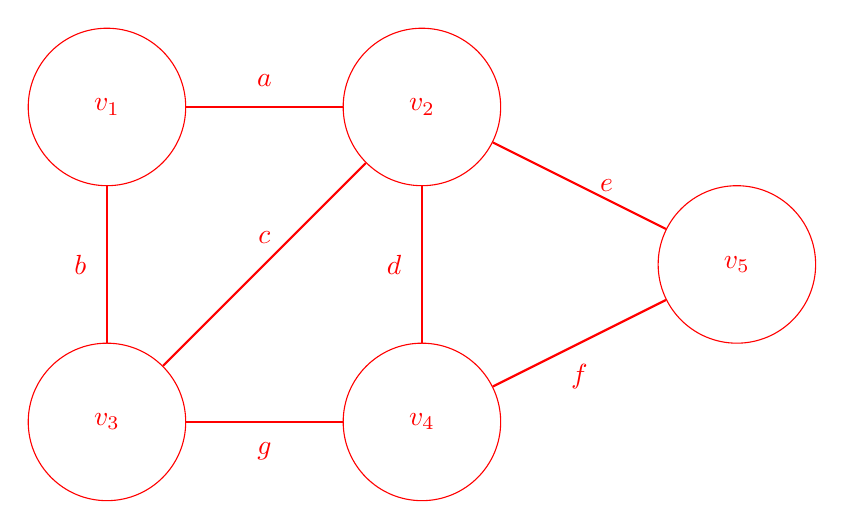
\begin{tikzpicture}[
nd/.style = {draw,circle,minimum size=2cm,red},
edge/.style = {thick,red}
]
  \node[nd] (v3) at (0,0) {$v_3$};
  \node[nd] (v1) at (0,4) {$v_1$};
  \node[nd] (v2) at (4,4) {$v_2$};
  \node[nd] (v4) at (4,0) {$v_4$};
  \node[nd] (v5) at (8,2) {$v_5$};
  
  \draw[edge] (v1) -- (v2) node [midway, label={$a$}] {};
  \draw[edge] (v1) -- (v3) node [midway, label=left:{$b$}] {};
  \draw[edge] (v3) -- (v2) node [midway, label=above:{$c$}] {};
  \draw[edge] (v4) -- (v2) node [midway, label=left:{$d$}] {};
  \draw[edge] (v2) -- (v5) node [midway, label=right:{$e$}] {};
  \draw[edge] (v5) -- (v4) node [midway, label=below:{$f$}] {};
  \draw[edge] (v3) -- (v4) node [midway, label=below:{$g$}] {};
\end{tikzpicture}
\end{document}
